% Intro - Guillaume
% I) Fonctionnalités
% 	1/ Le bureau - Hélène
% 		on peut ouvrir et fermer les fenetres
% 		pas de redimensionement
% 	2/ Les widgets - Elisoa
% 		a/ Calculatrice
% 		b/ Meteo statique
% 		c/ Galerie
% 		d/ Bloc-notes (zone de texte)
% 	3/ Les contraintes d'utilisation - Gregoire
% 		6 fenetres, 5 utilisateurs, ...
% II) Scénarios d'utilisation - Florian et Quentin
% 	ouvrir une fenetre, utiliser un widget, fermer une fenetre, ...
% Conclusion - Guillaume

% Relecture : Hélène


\documentclass[a4paper, 12pt]{report}
\usepackage[utf8]{inputenc}
\title{Document de spécifications \\ Bureau distribué}
\author{Hélène Soudry \and Elisoa Ramarokoto \and Quentin Diaferia \and Florian Lepetit \and Gregoire Gutzwiller \and Guillaume Minette De Saint-Martin}
\date{Février 2015}
\begin{document}
\maketitle
\tableofcontents
\chapter{Introduction}
\paragraph{}Dans le cadre du cours d'informatique répartie, nous réalisons un projet permettant la mise en pratique des connaissances acquises au cours de cet enseignement. Ce projet consiste en la réalisation d'un bureau distribué, c'est à dire un un MVC distribué appliqué à un bureau virtuel. 

Ce document est la concrétisation de la seconde étape de réalisation du projet, il marque la clôture de la phase de conception.

Nous détaillerons dans un premier temps les différents cas d'utilisation ensuite les diagrammes de séquence système, de classes participantes puis de classes et enfin d'interaction. nous finirons par la conception détaillée.   
\chapter{Fonctionnalités}
% Intro - Guillaume
% I) Fonctionnalités
% 	1/ Le bureau - Hélène
% 		on peut ouvrir et fermer les fenetres
% 		pas de redimensionement
% 	2/ Les widgets - Elisoa
% 		a/ Calculatrice
% 		b/ Meteo statique
% 		c/ Galerie
% 		d/ Bloc-notes (zone de texte)
% 	3/ Les contraintes d'utilisation - Gregoire
% 		6 fenetres, 5 utilisateurs, ...
% II) Scénarios d'utilisation - Florian et Quentin
% 	ouvrir une fenetre, utiliser un widget, fermer une fenetre, ...
% Conclusion - Guillaume

% Relecture : Hélène
\section{Le bureau}
Le bureau comportera un fond d'écran préalablement choisi et se trouvant sur le serveur. En bas de celui-ci, se trouvera une barre de lancement d'applications. Elle sera composé de 4 icônes, chaque icône correspondant à un widget. 

Lors du clic sur l'une de ces icônes, une nouvelle fenêtre apparaîtra à une position aléatoire sur le bureau. Une fenêtre ne pourra pas apparaître sur une autre. 

Il ne sera pas possible de redimensionner les fenêtres, cela pouvant causer des problème quant à l'apparition de nouveaux widgets. 

Il sera par contre possible de de fermer les fenêtres se trouvant sur le bureau sous condition d'être la personne ayant autorité sur celles-ci.

\section{Les widgets}
Le bureau propose quatre types de widgets : calculatrice, météo, galerie, bloc-notes.
{\color{red}
\subsection*{Calculatrice}

Ce widget est constitué d'un champ de saisie des calcul, d'un champ d'affichage du résultat d'un calcul et de boutons de saisie des chiffres ou opérateurs de calcul.

Il permet la réalisation de calculs simples : addition et soustraction d'entiers naturels.

Il permet également l'effacement de l'opération en cours de saisie à l'aide d'un bouton effacer qui efface la totalité de la ligne de saisie.

Le widget possède donc les éléments suivants :
\begin{itemize}
\item un bouton "+";
\item un bouton "-";
\item un bouton "effacer";
\item un pavé numérique.
\end{itemize}
}
\subsection*{Météo}
Ce widget indique la météo d'une ville en fournissant les informations suivantes : nom de la ville, température, tendance météorologique.

Une seule ville sera présentée par ce widget, Rouen, avec des données figées (sans mise à jour en temps réel) sur le serveur et non modifiables par les utilisateurs.

\subsection*{Galerie}
Ce widget est constitué d'une zone d'affichage des images et de boutons de navigation (gauche et droite) permettant le défilement des images de la galerie en boucle infinie.

Les images sont stockées sur le serveur et ne sont pas modifiables par les utilisateurs.

\subsection*{Bloc-notes}
Ce widget est constitué d'une zone de texte modifiable par une entrée standard au clavier et dans laquelle le positionnement peut être fait à l'aide d'une souris ou du pavé directionnel du clavier.
\section{Les contraintes d'utilisation}
Les performances du produit livré à l'issue du projet sont très 
importante. Le logiciel conçu devra, pour simuler une application
temps-réel, avoir un temps de réponse infiniment petit. Le temps
de réponse maximum est de 2 secondes (hors latence liée au réseau).

En outre, l'application en production doit supporter l'ouverture de 
six fenêtres au maximum et de trois utilisateurs connectés simultanément.

Pour des raisons légales, il sera impossible d'importer ses propres
photos dans la fenêtre de galerie de photos. L'application n'accèdera
ainsi à aucun moment aux données personnelles stockées sur les machines
des utilisateurs.

Lors du développement, une attention toute particulière sera portée
à la gestion du système de verrous sur des fenêtres. En effet, pour 
simplifier l'utilisation de l'application, les utilisateurs ne 
pourront pas avoir la main sur plus d'une fenêtre à la fois.

Suite à la demande du client, il est demandé de privilégier, tant que
possible, l'utilisation de méthodes liées à l'informatique répartie pour
la gestion du réseau dans l'application.


\chapter{Scénarios d'utilisation}
% L’utilisateur connecté au bureau virtuel pourra lancer un widget au travers d’un lanceur. Celui-ci s’apparentera au dock du système 
% d’exploitation Mac. Cela ne sera possible que si le nombre de widgets ouverts n’a pas atteint sa valeur maximale.

% L’utilisateur pourra ouvrir une fenêtre de type calculatrice et saisir une addition ou une soustraction. Le résultat apparaîtra sur 
% l’écran de tous les utilisateurs.

% Un utilisateur pourra aussi lancer le widget bloc-notes, permettant de saisir du texte et ainsi de l’afficher auprès des autres machines clientes.

% Un widget « Photos » pourra être utilisé afin de faire défiler quelques images pré-chargées sur le serveur.

% L’utilisateur connecté au bureau virtuel pourra quitter l’application via un bouton disponible dans le dock de lancement.

\section{Scénario d'utilisation 1}
\begin{itemize}
	\item Nom : Se connecter au serveur;
	\item Description : L'utilisateur accède au bureau virtuel via le programme correspondant;
	\item Acteurs : Utilisateur du bureau virtuel.
\end{itemize}

\paragraph{Séquence d'événements}
\begin{itemize}
	\item L'utilisateur lance le programme "bureau virtuel" sur son ordinateur personnel;
	\item Le serveur vérifie si le nombre d'utilisateurs ne dépasse pas la limite;
	\item L'utilisateur accède au bureau virtuel.
\end{itemize}

\paragraph{Exceptions}
\begin{itemize}
	\item L'utilisateur lance le programme;
	\item Le nombre d'utilisateur dépasse la limite;
	\item L'utilisateur est invité à réessayer de se connecter plus tard, lorsqu'un utilisateur se sera déconnecté.
\end{itemize}

% ------------------------------------

\section{Scénario d'utilisation 2}
\begin{itemize}
	\item Nom : Ouvrir une fenêtre;
	\item Description : L'utilisateur ouvre une des fenêtres disponibles sur le bureau;
	\item Acteurs : Utilisateur du bureau virtuel;
	\item Préalable : L'utilisateur est connecté au serveur.
\end{itemize}

\paragraph{Séquence d'événements}
\begin{itemize}
	\item L'utilisateur clique sur l'une des icônes disponibles représentant un widget;
	\item Le serveur vérifie que le nombre de fenêtres est inférieur à 6;
	\item Si le nombre de fenêtres ouvertes est inférieur à 6, le widget s'ouvre.
\end{itemize}

\paragraph{Exceptions}
\begin{itemize}
	\item L'utilisateur clique sur un lanceur;
	\item Le nombre de widgets ouverts est de 6 ou plus;
	\item Un message d'erreur apparaît invitant l'utilisateur à fermer une fenêtre pour en ouvrir une autre.
\end{itemize}

% ------------------------------------
{\color{red}
\section{Scénario d'utilisation 3}
\begin{itemize}
	\item Nom : Saisir une opération;
	\item Description : L'utilisateur saisit une opération sur le widget Calculatrice;
	\item Acteurs : Utilisateur du bureau virtuel;
	\item Préalable : L'utilisateur est connecté au serveur, un widget Calculatrice est ouvert.
\end{itemize}

\paragraph{Séquence d'événements}
\begin{itemize}
	\item L'utilisateur clique sur le bouton représentant le premier opérande;
	\item L'utilisateur clique sur le bouton représentant l'opérateur;
	\item L'utilisateur clique sur le bouton représentant le second opérande;
	\item L'utilisateur clique sur le symbole "=";
	\item Le résultat est affiché.
\end{itemize}
}

% ------------------------------------

\section{Scénario d'utilisation 4}
\begin{itemize}
	\item Nom : Regarder des photos;
	\item Description : L'utilisateur utilise le widget Galerie;
	\item Acteurs : Utilisateur du bureau virtuel;
	\item Préalable : L'utilisateur est connecté au serveur, un widget Galerie est ouvert.
\end{itemize}

\paragraph{Séquence d'événements}
\begin{itemize}
	\item L'utilisateur clique sur le bouton d'afficher l'image suivante;
	\item L'utilisateur clique sur le bouton d'afficher l'image précédente.
\end{itemize}


% ------------------------------------

\section{Scénario d'utilisation 5}
\begin{itemize}
	\item Nom : Quitter le bureau virtuel;
	\item Description : L'utilisateur se déconnecte du serveur;
	\item Acteurs : Utilisateur du bureau virtuel;
	\item Préalable : L'utilisateur est connecté  au serveur.
\end{itemize}

\paragraph{Séquence d'événements}
\begin{itemize}
	\item L'utilisateur clique sur le bouton "Déconnexion";
	\item Une fenêtre de confirmation s'ouvre demandant à l'utilisateur de cliquer sur "confirmer" ou "annuler";
	\item L'utilisateur clique sur "confirmer";
	\item L'utilisateur est déconnecté du serveur.
\end{itemize}

{\color{red}
Ce diagramme résume les différents cas d'utilisation définis dans le dossier de spécifications externes.

\begin{figure}[H]
	\centering
	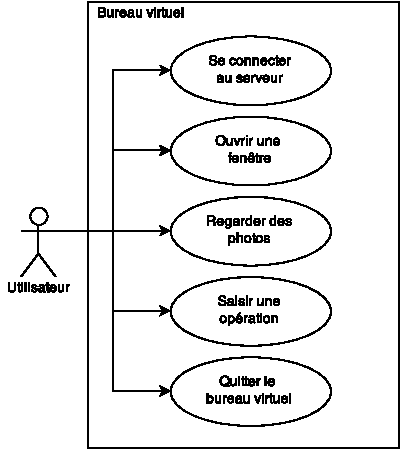
\includegraphics[scale=0.8]{diagrammes/DCU.pdf}
	\caption{Diagramme des cas d'utilisation}
\end{figure}
}
\chapter{Conclusion}
Le projet d'informatique répartie nous permet de développer un projet de A à Z. Il nous force à faire des choix technologiques en fonction des spécifications et de la conception que nous avons réalisé auparavant. De cette façon, ce projet nous a appris l'importance des étapes de conception et de spécification. 

Les premières étapes nous ont forcé à faire des choix de spécifications et de conception, ce qui est différent de la plupart des projets auxquels nous avons participé jusqu'ici.

La mise en pratique des concepts abordés lors des cours d'informatique répartie nous a permis de mieux comprendre les technologies utilisées. 
\end{document}